% ============================================================================
%  Design Review Presentation
%  Workload-Driven Custom RISC-V Instructions for Edge Video Anomaly Detection
%  Compile:  pdflatex design_review.tex   (run twice)   or   tectonic design_review.tex
% ============================================================================
\documentclass[aspectratio=169,11pt]{beamer}

\usetheme{Madrid}
\usecolortheme{default}
\definecolor{navy}{HTML}{1F3A5F}
\definecolor{accent}{HTML}{D1495B}
\definecolor{soft}{HTML}{EAF0F7}
\definecolor{okgreen}{HTML}{2E7D32}
\setbeamercolor{structure}{fg=navy}
\setbeamercolor{title}{fg=white,bg=navy}
\setbeamercolor{frametitle}{fg=white,bg=navy}
\setbeamercolor{block title}{fg=white,bg=navy}
\setbeamercolor{block body}{bg=soft}
\setbeamertemplate{navigation symbols}{}
\setbeamertemplate{itemize items}[circle]

\usepackage[T1]{fontenc}
\usepackage{booktabs}
\usepackage{array}
\usepackage{listings}
\usepackage{tikz}
\usetikzlibrary{arrows.meta,positioning,shapes.geometric,shapes.misc,fit,calc,backgrounds}

\lstset{basicstyle=\ttfamily\scriptsize,keywordstyle=\color{navy}\bfseries,
        commentstyle=\color{gray},columns=fullflexible,frame=single,
        backgroundcolor=\color{soft},breaklines=true,
        morekeywords={if,else,begin,end,rule,endrule,Bit,Reg,let}}

\tikzset{
  box/.style={draw=navy,thick,rounded corners=3pt,fill=soft,align=center,
              minimum height=8mm,inner sep=4pt,font=\small},
  hot/.style={box,fill=accent!18,draw=accent},
  arr/.style={-{Stealth[length=2.5mm]},thick,navy},
  darr/.style={{Stealth[length=2.5mm]}-{Stealth[length=2.5mm]},thick,navy},
  lbl/.style={font=\scriptsize,midway,fill=white,inner sep=1pt}
}

% ---- EDIT THESE ------------------------------------------------------------
\title[Custom RISC-V ISA for Edge Anomaly Detection]
      {Workload-Driven Custom RISC-V Instruction Extensions\\
       for Edge Video Anomaly Detection}
\subtitle{Design Review}
\author[Team 2]{Member 1 \and Member 2 \and Member 3 \and Member 4\\[2pt]
       {\small Guide: Jisha Robin}}
\institute[Dept. of CSE]{Department of Computer Science and Engineering}
\date{\today}
% ----------------------------------------------------------------------------

\begin{document}

% ============================================================================
\begin{frame}
  \titlepage
\end{frame}

\begin{frame}{Outline}
  \begin{columns}[T]
    \column{0.48\textwidth}
    \begin{enumerate}
      \item Introduction
      \item Problem Definition
      \item Objectives
      \item Functional \& Non-Functional Requirements
      \item Overall System Architecture
      \item Modules and Their Details
    \end{enumerate}
    \column{0.48\textwidth}
    \begin{enumerate}\setcounter{enumi}{6}
      \item Design Diagrams
      \item Workloads \& Test Data
      \item Risks \& Challenges
      \item Expected Output
      \item Conclusion
      \item References
    \end{enumerate}
  \end{columns}
\end{frame}

% ============================================================================
\section{Introduction}
\begin{frame}{Introduction: Why Edge AI for Surveillance?}
  \begin{columns}[T]
    \column{0.55\textwidth}
    \begin{itemize}
      \item Metro / CCTV networks need \textbf{continuous, real-time} anomaly
            detection: violence, falls, crowd panic, fire, abandoned luggage.
      \item Sending every frame to a server costs \textbf{latency, bandwidth
            and privacy}.
      \item \textbf{Edge inference}: run the neural network on a small device
            next to the camera.
      \item Edge CPUs are slow at the core CNN operation, the
            \textbf{multiply-accumulate (MAC)}, which runs millions of times per frame.
    \end{itemize}
    \column{0.42\textwidth}
    \centering
    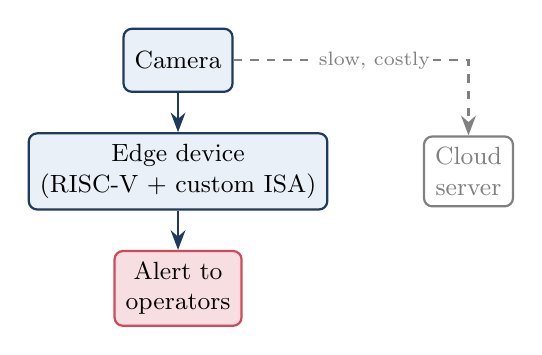
\begin{tikzpicture}[node distance=5mm]
      \node[box] (cam) {Camera};
      \node[box,below=of cam] (edge) {Edge device\\(RISC-V + custom ISA)};
      \node[hot,below=of edge] (alert) {Alert to\\operators};
      \draw[arr] (cam) -- (edge);
      \draw[arr] (edge) -- (alert);
      \node[box,right=12mm of edge,fill=white,draw=gray,text=gray] (srv) {Cloud\\server};
      \draw[arr,gray,dashed] (cam.east) -| node[lbl,pos=.3]{slow, costly} (srv);
    \end{tikzpicture}
  \end{columns}
\end{frame}

\begin{frame}{Introduction: RISC-V and the Shakti C-Class Core}
  \begin{columns}[T]
    \column{0.5\textwidth}
    \begin{block}{RISC-V}
      \begin{itemize}
        \item Open, royalty-free instruction set architecture (ISA)
        \item Opcode space reserved for \textbf{custom instructions}
              (\texttt{custom-0..3})
        \item Lets us add hardware operations tailored to a workload
      \end{itemize}
    \end{block}
    \column{0.46\textwidth}
    \begin{block}{Shakti C-Class (IIT Madras)}
      \begin{itemize}
        \item 64-bit \textbf{RV64IMAFDC}, in-order, 6-stage pipeline
        \item Hardware FPU (Berkeley HardFloat), caches, MMU, AXI4 bus
        \item Written in \textbf{Bluespec SystemVerilog}, a \textbf{soft core}
              (can be simulated or put on an FPGA)
        \item Chosen over PicoRV32: a real pipeline, Linux-capable,
              and extensible
      \end{itemize}
    \end{block}
  \end{columns}
  \vspace{2mm}
  \centering\small Simulation flow: BSV $\rightarrow$ \texttt{bsc} $\rightarrow$
  Verilog $\rightarrow$ Verilator $\rightarrow$ cycle-accurate model \texttt{bin/out}
\end{frame}

% ============================================================================
\section{Problem Definition}
\begin{frame}{Problem Definition}
  \begin{itemize}
    \item General-purpose embedded cores execute CNN kernels with scalar
          instructions: each MAC takes \textbf{11--18 cycles} on baseline Shakti.
    \item One MobileNetV2 + GRU inference (8 frames) takes
          \textbf{31.9 billion cycles} on baseline Shakti.
    \item On the existing Kria KV260 prototype (ARM + FPGA accelerator),
          \textbf{$\sim$82\% of the frame time} is the ARM CPU reshuffling data;
          the accelerator itself uses only $\sim$9\%.
  \end{itemize}
  \vspace{3mm}
  \begin{block}{Problem Statement}
    Design \textbf{workload-driven custom RISC-V instructions}, integrate them into
    the Shakti C-Class core, and deploy the core with an FPGA accelerator to
    speed up \textbf{edge video anomaly detection}, measured against an
    unmodified baseline.
  \end{block}
\end{frame}

% ============================================================================
\section{Objectives}
\begin{frame}{Objectives}
  \begin{enumerate}
    \item \textbf{Profile} the target workloads (MobileNetV2 + GRU, then
          TinyMetro-Net) on PC \emph{and} on the Shakti core itself.
    \item \textbf{Identify} the dominant kernels and the real hardware bottleneck.
    \item \textbf{Design} custom instructions in RISC-V custom opcode space.
    \item \textbf{Implement} them in the Shakti decoder and floating-point unit (RTL).
    \item \textbf{Verify} bit-exact results and backward compatibility
          (official riscv-tests).
    \item \textbf{Measure} speedup using hardware counters
          (\texttt{mcycle}, \texttt{minstret}).
    \item \textbf{Deploy} Shakti on the Kria KV260 FPGA in place of the ARM core,
          driving the INT8 accelerator.
    \item \textbf{Compare} edge (Shakti + accelerator) with server-based inference.
  \end{enumerate}
\end{frame}

% ============================================================================
\section{Requirements}
\begin{frame}{Functional \& Non-Functional Requirements}
  \begin{columns}[T]
    \column{0.49\textwidth}
    \begin{block}{Functional}
      \begin{itemize}\small
        \item Decode and execute new custom-opcode instructions
        \item Results \textbf{bit-identical} to standard RISC-V code
        \item Standard RV64IMAFDC behaviour unchanged
        \item Per-kernel cycle and instruction measurement
        \item Run the CNN kernels (conv, depthwise, pointwise, ReLU) on the core
        \item Interface with the FPGA accelerator over AXI4 \emph{(planned)}
      \end{itemize}
    \end{block}
    \column{0.49\textwidth}
    \begin{block}{Non-Functional}
      \begin{itemize}\small
        \item \textbf{Performance:} $\geq$1.5$\times$ kernel speedup
        \item \textbf{Correctness:} riscv-tests (\texttt{rv64uf-fmadd}) pass
        \item \textbf{Low overhead:} small hardware additions
        \item \textbf{Reproducibility:} open-source flow
              (bsc, Verilator, GCC 14)
        \item \textbf{Edge constraints:} limited memory
              (16\,KB D-cache), real-time frame rate
        \item \textbf{Maintainability:} documented, logged design decisions
      \end{itemize}
    \end{block}
  \end{columns}
\end{frame}

% ============================================================================
\section{System Architecture}
\begin{frame}{Overall System Architecture (Target Edge System)}
  \centering
  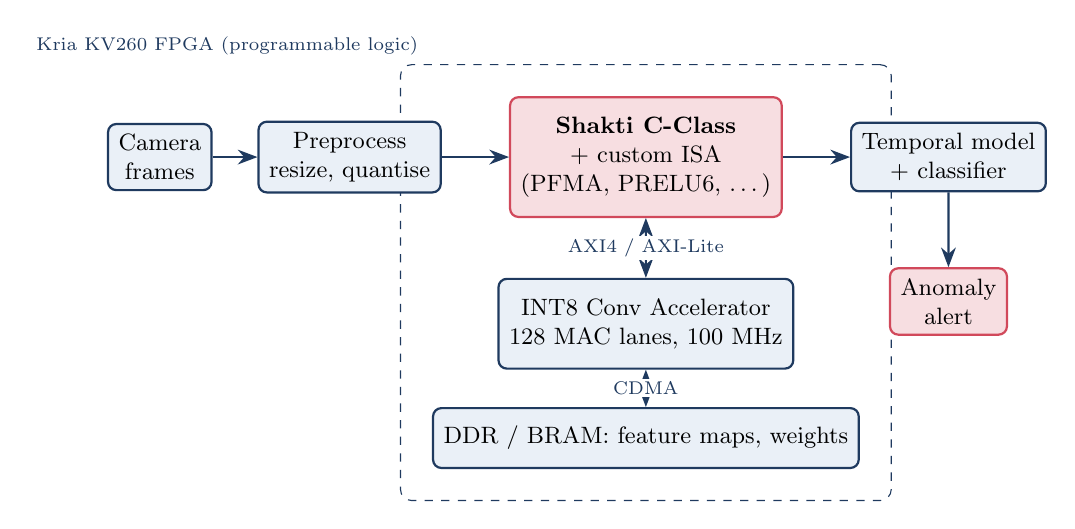
\begin{tikzpicture}[node distance=6mm and 6mm,scale=0.95,transform shape]
    \node[box] (cam) {Camera\\frames};
    \node[box,right=of cam] (pre) {Preprocess\\resize, quantise};
    \node[hot,right=9mm of pre,minimum width=32mm,minimum height=16mm] (cpu)
         {\textbf{Shakti C-Class}\\+ custom ISA\\(PFMA, PRELU6, \dots)};
    \node[box,below=8mm of cpu,minimum width=34mm,minimum height=12mm] (acc)
         {INT8 Conv Accelerator\\128 MAC lanes, 100 MHz};
    \node[box,below=5mm of acc] (mem) {DDR / BRAM: feature maps, weights};
    \node[box,right=9mm of cpu] (cls) {Temporal model\\+ classifier};
    \node[hot,below=10mm of cls] (out) {Anomaly\\alert};
    \draw[arr] (cam) -- (pre);
    \draw[arr] (pre) -- (cpu);
    \draw[darr] (cpu) -- node[lbl]{AXI4 / AXI-Lite} (acc);
    \draw[darr] (acc) -- node[lbl]{CDMA} (mem);
    \draw[arr] (cpu) -- (cls);
    \draw[arr] (cls) -- (out);
    \begin{scope}[on background layer]
      \node[draw=navy,dashed,rounded corners,fit=(cpu)(acc)(mem),inner sep=4mm,
            label={[font=\scriptsize,navy]above left:Kria KV260 FPGA (programmable logic)}] {};
    \end{scope}
  \end{tikzpicture}
  \par\vspace{1mm}
  {\small Shakti replaces the ARM Cortex-A53 as the host that drives the accelerator
  and runs the non-convolution work.}
\end{frame}

\begin{frame}{Architecture: Inside the Shakti C-Class Pipeline}
  \centering
  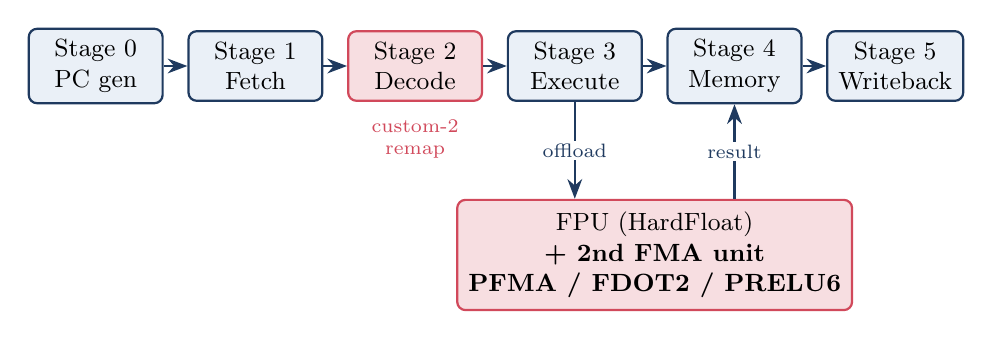
\begin{tikzpicture}[node distance=3mm]
    \node[box,minimum width=17mm] (s0) {Stage 0\\PC gen};
    \node[box,minimum width=17mm,right=of s0] (s1) {Stage 1\\Fetch};
    \node[hot,minimum width=17mm,right=of s1] (s2) {Stage 2\\Decode};
    \node[box,minimum width=17mm,right=of s2] (s3) {Stage 3\\Execute};
    \node[box,minimum width=17mm,right=of s3] (s4) {Stage 4\\Memory};
    \node[box,minimum width=17mm,right=of s4] (s5) {Stage 5\\Writeback};
    \foreach \a/\b in {s0/s1,s1/s2,s2/s3,s3/s4,s4/s5} \draw[arr] (\a) -- (\b);
    \node[hot,minimum width=50mm,minimum height=14mm] (fpu) at ($(s3)!0.5!(s4)+(0,-2.4)$)
         {FPU (HardFloat)\\\textbf{+ 2nd FMA unit}\\\textbf{PFMA / FDOT2 / PRELU6}};
    \draw[arr] (s3.south) -- node[lbl]{offload} (s3.south |- fpu.north);
    \draw[arr] (s4.south |- fpu.north) -- node[lbl]{result} (s4.south);
    \node[font=\scriptsize,text=accent,below=1mm of s2,align=center] {custom-2\\remap};
  \end{tikzpicture}
  \vspace{3mm}
  \begin{itemize}\small
    \item \textcolor{accent}{\textbf{Modified}}: \texttt{decoder.bsv},
          \texttt{decoder.defines}, \texttt{fpu\_hardfloat.bsv}
    \item Unchanged: fetch, scoreboard, forwarding, memory, writeback. The new
          instructions reuse the existing FLOAT path.
  \end{itemize}
\end{frame}

% ============================================================================
\section{Modules}
\begin{frame}{Module 1: Workload Profiling (PC $\rightarrow$ Shakti)}
  \begin{columns}[T]
    \column{0.44\textwidth}
    \small\textbf{PyTorch on a PC (MobileNetV2 + GRU)}\\[1mm]
    \begin{tabular}{lr}\toprule
      Operation & MACs / frame\\\midrule
      Pointwise 1$\times$1 & 267.9 M\\
      Depthwise 3$\times$3 & 20.7 M\\
      First conv 3$\times$3 & 10.8 M\\
      GRU (8 steps) & 9.4 M\\\bottomrule
    \end{tabular}
    \column{0.54\textwidth}
    \small\textbf{Measured on baseline Shakti (1 inference)}\\[1mm]
    \begin{tabular}{lrr}\toprule
      Operation & cyc/MAC & Share\\\midrule
      \textbf{Pointwise} & 11.7--13.9 & \textbf{83.8\%}\\
      Depthwise & 16.7 & 8.7\%\\
      First conv & 17.7 & 4.8\%\\
      ReLU6 & 14.3/elem & 2.2\%\\
      GRU & 12.0 & 0.4\%\\\midrule
      \textbf{Total} & & \textbf{31.9 B cyc}\\\bottomrule
    \end{tabular}
  \end{columns}
  \vspace{3mm}
  \begin{block}{Finding}
    Pointwise convolution dominates on the real target. The FP32 data type
    rules out an INT8-only design, and Shakti already has \texttt{fmadd.s},
    so a scalar custom MAC would add nothing.
  \end{block}
\end{frame}

\begin{frame}{Module 2: Custom Instruction Design}
  \small
  \begin{tabular}{@{}llp{6.6cm}l@{}}\toprule
    Instruction & fmt & Semantics & FPU op\\\midrule
    \texttt{FDOT2.S} & 00 & $fd = a_1 b_1 + (a_0 b_0 + c)$, 2 FMAs \emph{in sequence} & \texttt{0110}\\
    \texttt{PFMA.S}  & 10 & $fd = [\,x_1 w + c_1 \mid x_0 w + c_0\,]$, 2 FMAs \emph{in parallel} & \texttt{0111}\\
    \texttt{PRELU6.S}& 01 & $fd = [\,\mathrm{clamp}_{0..6}(x_1) \mid \mathrm{clamp}_{0..6}(x_0)\,]$, 1 cycle & \texttt{0101}\\\bottomrule
  \end{tabular}
  \vspace{3mm}
  \begin{itemize}
    \item All three use the \textbf{custom-2} opcode (\texttt{0x5B}) with the R4
          layout; fmt bits [26:25] select the instruction.
    \item Two FP32 values are \textbf{packed} into one 64-bit FP register
          (FLEN = 64).
    \item \textbf{Design path:} FDOT2 halved the instruction count but gave only
          1.07--1.13$\times$. That revealed the real bottleneck: the FPU accepts
          \textbf{one operation at a time} (about 10-cycle FMA latency).
          $\Rightarrow$ PFMA adds a \textbf{second FMA unit} so two MACs overlap.
  \end{itemize}
\end{frame}

\begin{frame}[fragile]{Module 3: Hardware Integration (RTL)}
  \begin{columns}[T]
    \column{0.47\textwidth}
    \small
    \begin{enumerate}
      \item \textbf{Decoder remap}: rewrite custom-2 into an internal FMADD form,
            so the existing decode, scoreboard and writeback are reused unchanged.
      \item \textbf{Own FPU opcode} (\texttt{fn}): the R4 \texttt{f7} field holds
            register data, not instruction bits.
      \item \textbf{Raw operands}: bypass NaN-boxing for packed values.
      \item \textbf{Second FMA unit} \texttt{spfma2} for PFMA lane 1.
      \item \textbf{PRELU6}: integer compares on IEEE bits, 1 cycle.
    \end{enumerate}
    \column{0.51\textwidth}
\begin{lstlisting}
// decoder.bsv (fn_decode)
if (inst_in[6:0] == 'b1011011)
  inst = {inst_in[31:27], 2'b10,
          inst_in[24:7], 7'b1000011};

// fpu_hardfloat.bsv (rule start)
if (opcode == 4'b0111) begin  // PFMA
  spfma.request (0, r1[31:0],
                 r2[31:0], r3[31:0],  f3);
  spfma2.request(0, r1[63:32],
                 r2[31:0], r3[63:32], f3);
  rg_pfma <= True;
end
\end{lstlisting}
  \end{columns}
\end{frame}

\begin{frame}{Module 4: Verification \& Benchmarking}
  \begin{columns}[T]
    \column{0.5\textwidth}
    \begin{block}{Verification}
      \begin{itemize}\small
        \item Directed test: FDOT2 of $[2,1.5]\cdot[4,3]+0.5 = 13.0$ \checkmark
        \item Every benchmark checks \textbf{bit-exact} equality with the
              baseline C code
        \item Official \texttt{rv64uf/fmadd.S} passes after each change
        \item Pass/fail read from \texttt{tohost}; traces in \texttt{rtl.dump}
      \end{itemize}
    \end{block}
    \column{0.46\textwidth}
    \begin{block}{Bugs found \& fixed}
      \begin{itemize}\small
        \item Stale decoder build (illegal-instruction trap)
        \item NaN-boxing turned packed inputs into NaN
        \item Wrong source for the FPU \texttt{f7} field
        \item BSC rule conflict: request and response in one rule
      \end{itemize}
    \end{block}
  \end{columns}
  \vspace{2mm}
  \centering\small Benchmark flow: C kernel $\rightarrow$ RISC-V GCC $\rightarrow$
  \texttt{elf2hex} $\rightarrow$ simulated Shakti $\rightarrow$
  \texttt{mcycle}/\texttt{minstret} $\rightarrow$ report
\end{frame}

\begin{frame}{Module 4: Measured Results (all bit-exact)}
  \centering\small
  \begin{tabular}{lccc}\toprule
    Kernel & Baseline & Custom & Speedup\\\midrule
    Pointwise, small K (16--144 ch) & 11.1--11.8 cyc/MAC & 6.6--7.0 & \textbf{1.69--1.70$\times$}\\
    Pointwise, large K (320--960 ch) & 13.8--13.9 cyc/MAC & 9.2--9.3 & \textbf{1.49--1.50$\times$}\\
    Depthwise 3$\times$3 (with pair copy) & 16.99 cyc/MAC & 10.86 & \textbf{1.56$\times$}\\
    First conv 3$\times$3, stride 2 & 18.28 cyc/MAC & 9.22 & \textbf{1.98$\times$}\\
    ReLU6 (PRELU6) & 14.00 cyc/elem & 3.52 & \textbf{3.98$\times$}\\\bottomrule
  \end{tabular}
  \vspace{4mm}
  \begin{tabular}{lrr}\toprule
    Whole MobileNetV2 + GRU inference (estimate) & Cycles & Speedup\\\midrule
    Baseline Shakti & 31.9 B & 1.00$\times$\\
    + PFMA (pointwise, depthwise, first conv) & 19.8 B & 1.61$\times$\\
    \textbf{+ PRELU6} & \textbf{19.3 B} & \textbf{1.66$\times$}\\\bottomrule
  \end{tabular}
\end{frame}

\begin{frame}{Module 5: FPGA Integration (Kria KV260)}
  \begin{columns}[T]
    \column{0.52\textwidth}
    \small\textbf{Existing prototype (SqueezeNet + TCN, INT8)}
    \begin{itemize}\small
      \item ARM Cortex-A53 (PYNQ / Python) + FPGA conv accelerator
      \item 128 INT8 MAC lanes at 100 MHz, AXI CDMA, three 1024-bit BRAMs
      \item Validated bit-exact on the board: 0 mismatches in 788,544 outputs
    \end{itemize}
    \column{0.45\textwidth}
    \small\textbf{Measured per frame on the board}\\[1mm]
    \begin{tabular}{lr}\toprule
      Output rebuild (ARM) & 1.29 s\\
      Max-pool (ARM) & 0.31 s\\
      \textbf{Accelerator conv} & \textbf{0.18 s}\\
      DMA + staging & 0.04 s\\\midrule
      Total per frame & 1.94 s\\\bottomrule
    \end{tabular}
  \end{columns}
  \vspace{3mm}
  \begin{block}{Plan}
    Replace the ARM with the Shakti soft core on the FPGA, port the host driver to
    bare-metal C, and target the CPU-side bottleneck (data reshuffling, pooling,
    requantisation) with custom instructions.
  \end{block}
\end{frame}

\begin{frame}{Module 6: Target Model: TinyMetro-Net (Team 1)}
  \begin{columns}[T]
    \column{0.5\textwidth}
    \begin{itemize}\small
      \item 13 layers (12 conv + 1 linear), \textbf{48,600 INT8 parameters}
            (47 KB)
      \item Conv 3$\times$3 + 5 $\times$ (depthwise s2 + pointwise) + final
            pointwise
      \item Requantisation:
            $\mathit{out} = \mathrm{clip}\big((\mathit{acc}\cdot s) \gg 15,\,0,\,127\big)$
      \item 8 classes (violence, falls, crowd, wrong-way, trespass, luggage,
            fire, normal)
    \end{itemize}
    \column{0.46\textwidth}
    \small\textbf{Where the work is (our calculation)}\\[1mm]
    \begin{tabular}{lrr}\toprule
      Part & MACs & Share\\\midrule
      \textbf{conv1} & \textbf{8.13 M} & \textbf{57\%}\\
      Pointwise $\times$6 & 5.04 M & 35\%\\
      Depthwise $\times$5 & 1.03 M & 7\%\\\midrule
      Total & 14.2 M & \\\bottomrule
    \end{tabular}
  \end{columns}
  \vspace{3mm}
  \small\textbf{Next:} a Shakti profile of TinyMetro, then INT8 instructions:
  a packed INT8 dot product (\texttt{PDOT8}) and a fused requantise + ReLU.
\end{frame}

% ============================================================================
\section{Design Diagrams}
\begin{frame}{Activity Diagram: Workload-Driven Design Method}
  \centering
  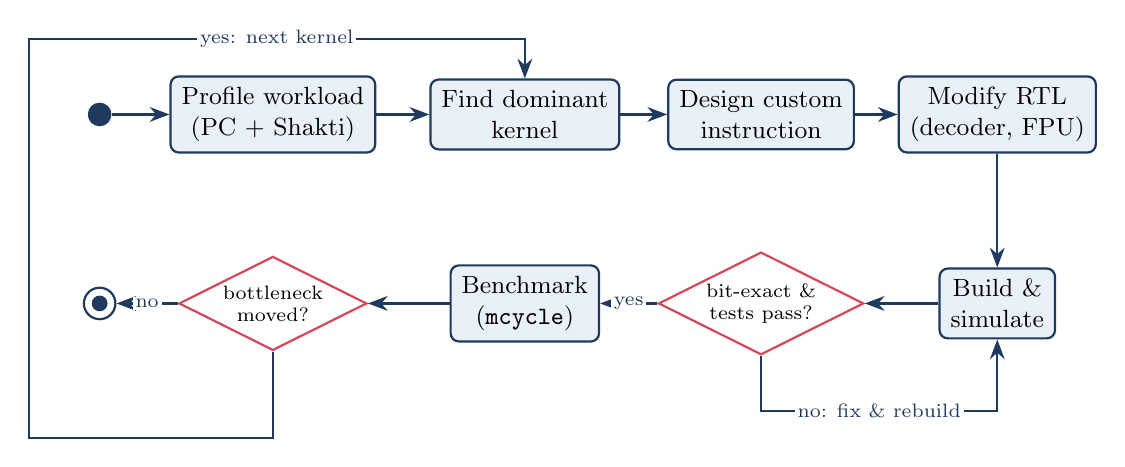
\begin{tikzpicture}[font=\small]
    \tikzset{dec/.style={diamond,draw=accent,thick,aspect=2,inner sep=1pt,
             font=\scriptsize,align=center,fill=white}}
    \node[circle,fill=navy,minimum size=3mm,inner sep=0] (st) at (0,0) {};
    \node[box] (a1) at (2.2,0)  {Profile workload\\(PC + Shakti)};
    \node[box] (a2) at (5.4,0)  {Find dominant\\kernel};
    \node[box] (a3) at (8.4,0)  {Design custom\\instruction};
    \node[box] (a4) at (11.4,0) {Modify RTL\\(decoder, FPU)};
    \node[box] (a5) at (11.4,-2.4) {Build \&\\simulate};
    \node[dec] (d1) at (8.4,-2.4) {bit-exact \&\\tests pass?};
    \node[box] (a6) at (5.4,-2.4) {Benchmark\\(\texttt{mcycle})};
    \node[dec] (d2) at (2.2,-2.4) {bottleneck\\moved?};
    \node[circle,draw=navy,thick,minimum size=4mm] (en) at (0,-2.4) {};
    \node[circle,fill=navy,minimum size=2mm,inner sep=0] at (en) {};
    \draw[arr] (st) -- (a1); \draw[arr] (a1) -- (a2); \draw[arr] (a2) -- (a3);
    \draw[arr] (a3) -- (a4); \draw[arr] (a4) -- (a5); \draw[arr] (a5) -- (d1);
    \draw[arr] (d1) -- node[lbl]{yes} (a6);
    \draw[arr] (a6) -- (d2);
    \draw[arr] (d2) -- node[lbl]{no} (en);
    \draw[arr] (d1.south) -- ++(0,-0.7) -| node[lbl,pos=.25]{no: fix \& rebuild} (a5.south);
    \draw[arr] (d2.south) -- ++(0,-1.1) -- ++(-3.1,0) |- ($(a2.north)+(0,0.5)$)
               node[lbl,pos=.75]{yes: next kernel} -- (a2.north);
  \end{tikzpicture}
\end{frame}

\begin{frame}{Sequence Diagram: Executing One \texttt{PFMA.S} Instruction}
  \centering
  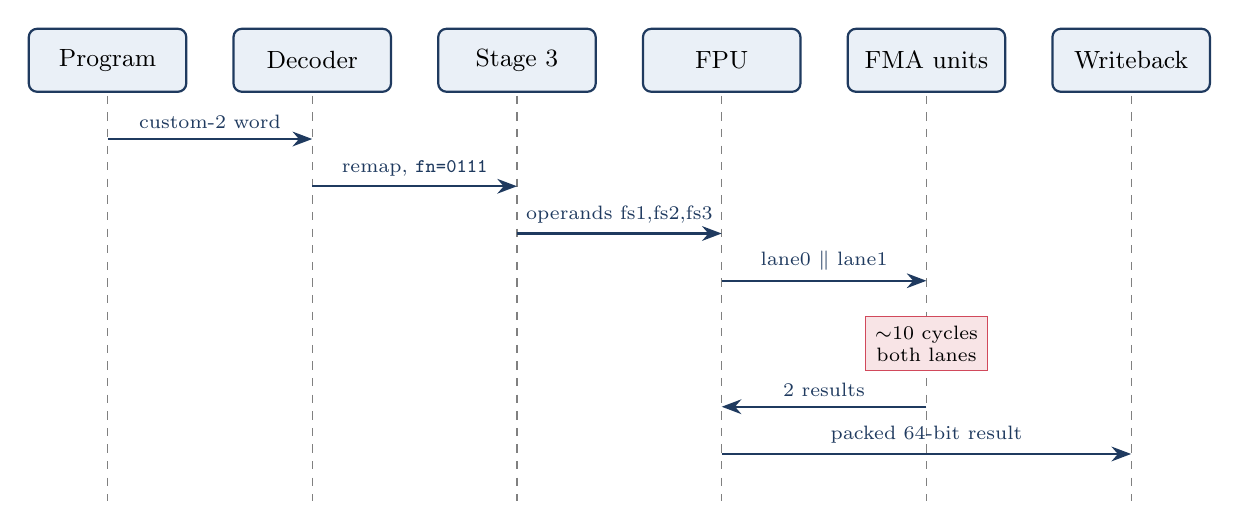
\begin{tikzpicture}[font=\small]
    \foreach \x/\n/\t in {0/p/Program,2.6/d/Decoder,5.2/e/Stage 3,7.8/f/FPU,10.4/u/FMA units,13/w/Writeback}{
      \node[box,minimum width=20mm] (\n) at (\x,0) {\t};
      \draw[dashed,gray] (\x,-0.45) -- (\x,-5.6);
    }
    \draw[arr] (0,-1.0) -- node[above,font=\scriptsize]{custom-2 word} (2.6,-1.0);
    \draw[arr] (2.6,-1.6) -- node[above,font=\scriptsize]{remap, \texttt{fn=0111}} (5.2,-1.6);
    \draw[arr] (5.2,-2.2) -- node[above,font=\scriptsize]{operands fs1,fs2,fs3} (7.8,-2.2);
    \draw[arr] (7.8,-2.8) -- node[above,font=\scriptsize]{lane0 $\parallel$ lane1} (10.4,-2.8);
    \node[draw=accent,fill=accent!15,font=\scriptsize,align=center] at (10.4,-3.6) {$\sim$10 cycles\\both lanes};
    \draw[arr] (10.4,-4.4) -- node[above,font=\scriptsize]{2 results} (7.8,-4.4);
    \draw[arr] (7.8,-5.0) -- node[above,font=\scriptsize]{packed 64-bit result} (13,-5.0);
  \end{tikzpicture}
\end{frame}

\begin{frame}{Data Flow Diagram (Level 1): Anomaly Detection Pipeline}
  \centering
  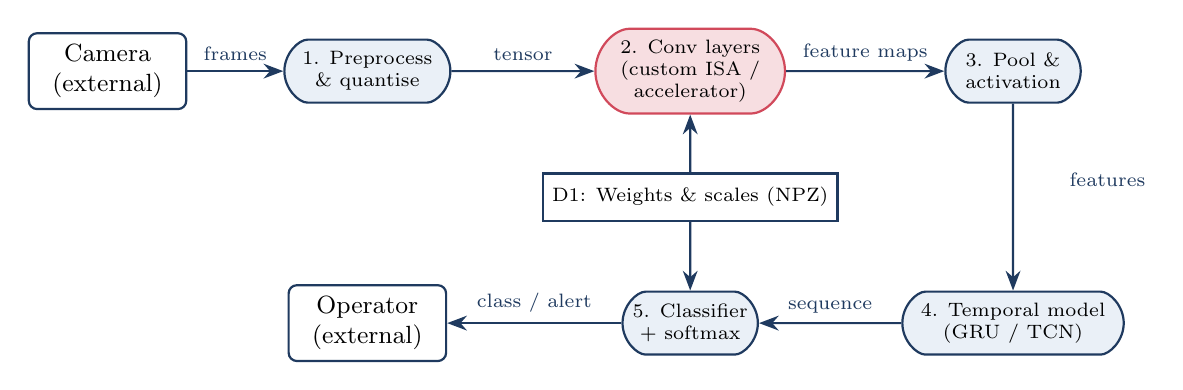
\begin{tikzpicture}[font=\small]
    \tikzset{proc/.style={box,rounded rectangle,minimum width=20mm,font=\scriptsize},
             ext/.style={box,fill=white,minimum width=20mm},
             fl/.style={font=\scriptsize,above,midway}}
    \node[ext]  (cam) at (0,0)      {Camera\\(external)};
    \node[proc] (p1)  at (3.3,0)    {1. Preprocess\\\& quantise};
    \node[proc,fill=accent!18,draw=accent] (p2) at (7.4,0) {2. Conv layers\\(custom ISA /\\accelerator)};
    \node[proc] (p3)  at (11.5,0)   {3. Pool \&\\activation};
    \node[proc] (p4)  at (11.5,-3.2) {4. Temporal model\\(GRU / TCN)};
    \node[proc] (p5)  at (7.4,-3.2)  {5. Classifier\\+ softmax};
    \node[ext]  (op)  at (3.3,-3.2)  {Operator\\(external)};
    \node[draw=navy,thick,fill=white,minimum width=30mm,minimum height=6mm,font=\scriptsize]
          (ds) at (7.4,-1.6) {D1: Weights \& scales (NPZ)};
    \draw[arr] (cam) -- node[fl]{frames} (p1);
    \draw[arr] (p1) -- node[fl]{tensor} (p2);
    \draw[arr] (p2) -- node[fl]{feature maps} (p3);
    \draw[arr] (p3) -- node[fl,right,above=0pt,xshift=12mm]{features} (p4);
    \draw[arr] (p4) -- node[fl]{sequence} (p5);
    \draw[arr] (p5) -- node[fl]{class / alert} (op);
    \draw[arr] (ds) -- (p2);
    \draw[arr] (ds) -- (p5);
  \end{tikzpicture}
\end{frame}

\begin{frame}{Use Case Diagram}
  \centering
  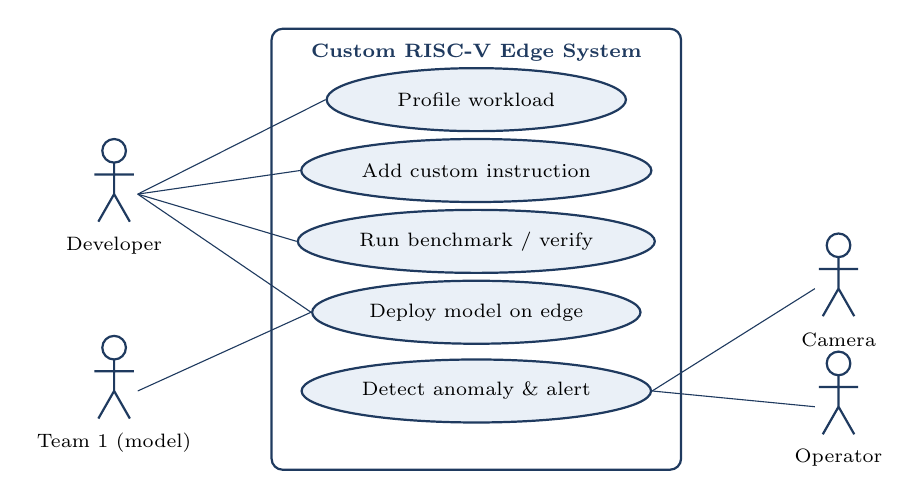
\begin{tikzpicture}[font=\small]
    \tikzset{actor/.pic={\draw[thick,navy] (0,0.55) circle (0.15);
        \draw[thick,navy] (0,0.4) -- (0,0) (-0.25,0.25) -- (0.25,0.25)
                          (0,0) -- (-0.2,-0.35) (0,0) -- (0.2,-0.35);},
             uc/.style={ellipse,draw=navy,thick,fill=soft,minimum width=38mm,
                        minimum height=8mm,font=\scriptsize}}
    \draw[navy,thick,rounded corners] (-2.6,-3.2) rectangle (2.6,2.4);
    \node[font=\scriptsize\bfseries,navy] at (0,2.1) {Custom RISC-V Edge System};
    \node[uc] (u1) at (0,1.5)  {Profile workload};
    \node[uc] (u2) at (0,0.6)  {Add custom instruction};
    \node[uc] (u3) at (0,-0.3) {Run benchmark / verify};
    \node[uc] (u4) at (0,-1.2) {Deploy model on edge};
    \node[uc] (u5) at (0,-2.2) {Detect anomaly \& alert};
    \pic at (-4.6,0.3) {actor}; \node[font=\scriptsize] at (-4.6,-0.35) {Developer};
    \pic at (4.6,-0.9) {actor}; \node[font=\scriptsize] at (4.6,-1.55) {Camera};
    \pic at (4.6,-2.4) {actor}; \node[font=\scriptsize] at (4.6,-3.05) {Operator};
    \pic at (-4.6,-2.2) {actor}; \node[font=\scriptsize] at (-4.6,-2.85) {Team 1 (model)};
    \foreach \u in {u1,u2,u3,u4} \draw[navy] (-4.3,0.3) -- (\u.west);
    \draw[navy] (-4.3,-2.2) -- (u4.west);
    \draw[navy] (4.3,-0.9) -- (u5.east);
    \draw[navy] (4.3,-2.4) -- (u5.east);
  \end{tikzpicture}
\end{frame}

% ============================================================================
\section{Workloads}
\begin{frame}{Workloads \& Test Data}
  \small
  \begin{tabular}{@{}>{\raggedright\arraybackslash}p{3.3cm}>{\raggedright\arraybackslash}p{2.0cm}>{\raggedright\arraybackslash}p{8.2cm}@{}}\toprule
    Workload & Data type & Data used\\\midrule
    MobileNetV2 + GRU & FP32 & ImageNet-pretrained MobileNetV2; 8-frame
      sequences of 224$\times$224; random inputs for timing\\
    SqueezeNet 1.1 + TCN & INT8 & Kria package: \texttt{anomaly\_sample.mp4},
      \texttt{normal\_sample.mp4}; 16 sampled frames\\
    TinyMetro-Net (Team 1) & INT8 & 8-class metro dataset: 224 test frames,
      527 validation frames, 54 held-out clips\\\bottomrule
  \end{tabular}
  \vspace{3mm}
  \begin{itemize}
    \item Cycle timing does not depend on the data values, so profiling uses
          real layer shapes with synthetic data.
    \item Correctness is checked bit for bit against the baseline implementation.
  \end{itemize}
\end{frame}

% ============================================================================
\section{Risks}
\begin{frame}{Risks \& Challenges}
  \begin{columns}[T]
    \column{0.49\textwidth}
    \begin{itemize}\small
      \item \textbf{Non-pipelined FPU}: one operation at a time limits the total
            speedup to $\sim$1.66$\times$ (Amdahl's law)
      \item \textbf{Simulation speed}: a full network takes days in Verilator,
            so we measure sampled layers and extrapolate
      \item \textbf{Memory}: the 16\,KB D-cache slows the large layers
    \end{itemize}
    \column{0.49\textwidth}
    \begin{itemize}\small
      \item \textbf{FPGA integration}: no Vivado project yet; fitting Shakti and
            the accelerator on the K26 is unverified
      \item \textbf{Software port}: the Python driver must become bare-metal C
      \item \textbf{Data type}: target models are INT8, while our first
            instructions are FP32
      \item \textbf{Tooling}: stale builds, long rebuilds (15--20 min)
    \end{itemize}
  \end{columns}
\end{frame}

% ============================================================================
\section{Expected Output}
\begin{frame}{Expected Output: Achieved So Far}
  \centering
  \begin{tabular}{lcl}\toprule
    Deliverable & Status & Result\\\midrule
    PyTorch + Shakti profiling & \textcolor{okgreen}{\checkmark} & pointwise = 84\% of the time\\
    FDOT2.S & \textcolor{okgreen}{\checkmark} & 1.87$\times$ fewer instructions, 1.07--1.13$\times$\\
    PFMA.S (2nd FMA unit) & \textcolor{okgreen}{\checkmark} & 1.5--2.0$\times$ on conv kernels\\
    PRELU6.S & \textcolor{okgreen}{\checkmark} & 3.98$\times$ on ReLU6\\
    Regression (riscv-tests) & \textcolor{okgreen}{\checkmark} & all pass, bit-exact\\
    Whole-model estimate & \textcolor{okgreen}{\checkmark} & 31.9 B $\rightarrow$ 19.3 B cycles (\textbf{1.66$\times$})\\
    Kria prototype analysis & \textcolor{okgreen}{\checkmark} & bottleneck = ARM data handling\\\bottomrule
  \end{tabular}
\end{frame}

\begin{frame}{Expected Output: Final System}
  \begin{enumerate}
    \item \textbf{Pipelined FPU}: a new FMA every cycle (projected pointwise
          $\sim$2--3 cyc/MAC, $\sim$3--4$\times$ overall; to be measured)
    \item \textbf{INT8 instructions} for TinyMetro-Net: packed dot product,
          fused requantise + ReLU
    \item \textbf{Complete network} running on the customised Shakti core,
          compared end to end with baseline Shakti
    \item \textbf{Shakti + accelerator on the Kria KV260}, replacing the ARM core
    \item \textbf{Edge vs server} comparison of latency and throughput
  \end{enumerate}
  \vspace{2mm}
  \begin{block}{Comparison table (final report)}
    \centering\small
    Baseline Shakti \quad vs \quad Shakti + custom ISA \quad vs \quad
    ARM + accelerator \quad vs \quad Shakti + accelerator \quad vs \quad Server
  \end{block}
\end{frame}

% ============================================================================
\section{Conclusion}
\begin{frame}{Conclusion}
  \begin{itemize}
    \item A \textbf{workload-driven} method (profile $\rightarrow$ bottleneck
          $\rightarrow$ instruction $\rightarrow$ verify $\rightarrow$ measure)
          produced real, measured gains on an open RISC-V core.
    \item Three custom instructions (FDOT2, PFMA, PRELU6) were designed, built
          into Shakti C-Class and verified \textbf{bit-exact}, with standard ISA
          behaviour unchanged.
    \item Estimated \textbf{1.66$\times$} speedup for MobileNetV2 + GRU; the
          remaining bottleneck (the non-pipelined FPU) is identified and quantified.
    \item Next: INT8 instructions for Team 1's TinyMetro-Net, and deploying
          Shakti with the FPGA accelerator on the Kria KV260.
  \end{itemize}
\end{frame}

% ============================================================================
\section{References}
\begin{frame}[allowframebreaks]{References}
  \footnotesize
  \begin{enumerate}
    \item A. Waterman, K. Asanovi\'c (eds.), \emph{The RISC-V Instruction Set
          Manual, Volume I: Unprivileged ISA}, RISC-V International.
    \item SHAKTI Processor Program, IIT Madras, \emph{C-Class Core Documentation},
          \texttt{gitlab.com/shaktiproject/cores/c-class}.
    \item M. Sandler \emph{et al.}, ``MobileNetV2: Inverted Residuals and Linear
          Bottlenecks,'' \emph{CVPR}, 2018.
    \item K. Cho \emph{et al.}, ``Learning Phrase Representations using RNN
          Encoder--Decoder for Statistical Machine Translation,'' \emph{EMNLP}, 2014.
    \item F. Iandola \emph{et al.}, ``SqueezeNet: AlexNet-level accuracy with 50x
          fewer parameters and $<$0.5MB model size,'' arXiv:1602.07360, 2016.
    \item S. Bai, J. Z. Kolter, V. Koltun, ``An Empirical Evaluation of Generic
          Convolutional and Recurrent Networks for Sequence Modeling,''
          arXiv:1803.01271, 2018.
    \item J. Hauser, \emph{Berkeley HardFloat} floating-point hardware library.
    \item R. Nikhil, \emph{BSV by Example}, Bluespec Inc.
    \item W. Snyder, \emph{Verilator} open-source SystemVerilog simulator.
    \item J. Hennessy, D. Patterson, \emph{Computer Architecture: A Quantitative
          Approach}, 6th ed., Morgan Kaufmann, 2017.
    \item AMD/Xilinx, \emph{Kria KV260 Vision AI Starter Kit User Guide} and
          PYNQ documentation.
    \item Team 1, \emph{TinyMetro-Net: Architecture \& Hardware Specification},
          internal report, v1.0.
  \end{enumerate}
\end{frame}

\begin{frame}
  \centering
  \Huge\textcolor{navy}{Thank You}\\[4mm]
  \large Questions?
\end{frame}

\end{document}
